The conversion process used by \texfourht\ involves several tools
(see section \ref{sec:overview}, \nameref{sec:overview} for details). To
simplify the process, several alternative tools are used. The traditional tool
is the \shellcmd{htlatex} script and several other scripts working on the same
principle. Recommended tool that supersedes them is \shellcmd{make4ht}.


The translation of a LaTeX source file into HTML involves of loading tex4ht.sty
and *.4ht style files, choosing the desirable options for the translation,
compiling the source into dvi code with the native LaTeX engine, and
post-processing the outcome with the tex4ht and t4ht programs.

\section{\texttt{htlatex} and other conversion scripts}

The conversion command loads a script which takes on itself to invoke the
different steps of the process, without user intervention. The command assumes
the form

\begin{shellcommand}
htlatex filename "options1" "option2" "options3" "options4"
\end{shellcommand}

where the first set of options is for the tex4ht.sty and *.4ht style files, the
second set is for the tex4ht post-processor, the third for the t4ht
post-processor, and the last one is for the \LaTeX\ compiler. 


For instance:

\begin{shellcommand}
htlatex filename
\end{shellcommand}

This command requests a translation according to the default conditions, which are set to produce HTML transitional 4.0 code. 

\begin{shellcommand}
htlatex filename "html,2,info"
\end{shellcommand}

This command is equivalent to the previous one, specifying explicitly the option html for tex4ht.sty instead of doing so implicitly.

In addition, the command requests a break up of the output into separate web pages, in accordance to the two top sectioning levels of the document.

Moreover, it asks for a listing in the log file of the information available
for the style files in use. That information, among other things, also
introduces additional values available for the first list of options.

\begin{shellcommand}
htlatex filename "foo,frames" "" "-p"
\end{shellcommand}

This command requests LaTeX to load a \nameref{sec:private-configuration}, named
foo.cfg, and to place the content and table of contents in separate frames. In
addition, it asks t4ht not to produce bitmaps for pictures. 

\begin{shellcommand}
htlatex filename "html,charset=utf-8" "-cunihtf -utf8"
\end{shellcommand}

This command will produce HTML file in UTF 8 encoding. 

\section{\texttt{make4ht} build system}

\shellcmd{make4ht} can be used in a similar way:

\begin{shellcommand}
make4ht [make4ht options] filename "options1" "option2" "options3" "options4"
\end{shellcommand}

In contrast to \shellcmd{htlatex}, \shellcmd{make4ht} supports short options
that can simplify the command invocation. For example the following command may
be used for the UTF-8 output, which is preferable for most texts produced
today:

\begin{shellcommand}
make4ht -u filename
\end{shellcommand}

The default output format used by \shellcmd{make4ht} is HTML 5, which another
difference to \shellcmd{htlatex}. We will use only \shellcmd{make4ht} in the
following text.


\section{Overview of the Translation Process}\label{sec:overview}



The system can be activated with a sequence of commands of the following form, typically embedded within a script.

\begin{shellcommand}
latex      x            (or ‘tex x’) 
latex      x 
latex      x 
tex4ht     x 
t4ht       x 
\end{shellcommand}

The three compilations with La(TeX) are needed to ensure proper links. The approach is illustrated in the picture \ref{fig:process}. 

\begin{figure}
  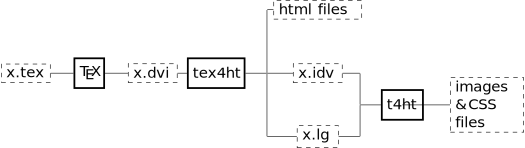
\includegraphics[width=\textwidth]{images/tex4ht_process/tex4ht_process}
  \caption{\texfourht\ process overview}
  \label{fig:process}
\end{figure}

\begin{description}
  \item[x.tex]

This is a source TeX/LaTeX/OtherTeX file that imports the style files tex4ht.sty and *.4ht. The style files define the features for the output.

\item[tex4ht]

The output of \TeX{} is a standard dvi file interleaved with special
instructions for the postprocessor \shellcmd{tex4ht} to use. The special
instructions come from implicit and explicit requests made in the source file
through commands of \texfourht.

The utility tex4ht translates the dvi code into standard text, while obeying
the requests it gets from the special instructions. The special instructions
may request the creation of files, insertion of html code, filtering of
pictures, and so forth.

In the extreme case that the source code contains no commands of TeX4ht, tex4ht
gets pure dvi code and it outputs (almost) plain text with no hypertext
elements in it.

The special (\texcommand{\special}) instructions seeded in the dvi code are not understood
by dvi processors other than those of TeX4ht.

\item[x.idv]

This is a dvi file extracted from x.dvi, and it contains the pictures needed in
the html files.

\item[x.lg]

This is a log file listing the pictures of x.idv, the png files that should be
created, CSS information, and user directives introduced through the
‘\texcommand{\Needs{...}}’ command.

\item[t4ht]
This is an interpreter for executing the requests made in the x.lg script.

\end{description}


